\documentclass[11pt,a4paper]{article}
\usepackage[margin=1in]{geometry}
\usepackage{graphicx}
\usepackage{booktabs}
\usepackage{longtable}
\usepackage{amsmath,amssymb}
\usepackage{hyperref}
\usepackage{setspace}
\usepackage{tikz}
\usetikzlibrary{shapes,arrows.meta,positioning}
\usepackage{caption}
\usepackage{subcaption}
\usepackage{enumitem}
\usepackage{url}
\usepackage{tabularx}
 % он у тебя уже есть
\graphicspath{{../results/figures/}{results/figures/}{./results/figures/}}

\title{Machine Learning and Deep Learning\\Integrated Course Project (Assignment 2)}
\author{Amirkhan Oral and Sardor Khassanov\\Student ID: 241695 and  240579 }
\date{May 2026}

\begin{document}
\maketitle
\begin{abstract}
This report documents six integrated tasks spanning classical classification, dimensionality reduction, multilayer perceptrons, convolutional neural networks, and a reflective survey of modern deep learning architectures. All experiments are implemented in Python with reproducible scripts under \texttt{src/}, exported figures under \texttt{results/figures/}, and structured notebooks under \texttt{notebooks/}. Run pipelines from the project root before compiling this document so that figure paths resolve.
\end{abstract}
\onehalfspacing
\tableofcontents
\newpage

\section{Task 1 --- Classification Algorithms}

\subsection{Theoretical summaries}

\subsubsection{k-Nearest Neighbors (k-NN)}
k-NN is a non-parametric, instance-based classifier. A test point receives the majority label among the $k$ closest training examples under a metric (typically Euclidean or Minkowski). The decision boundary is piecewise linear in feature space and adapts locally to data density. Key hyperparameters include $k$ (bias--variance trade-off: small $k$ increases variance and sensitivity to noise; large $k$ smooths boundaries), the distance metric and optional feature weighting, and sometimes distance-weighted voting. Training is trivial ($O(1)$) aside from storing data, but storage is $O(n d)$ for $n$ samples in $d$ dimensions; inference requires $O(n d)$ per query without advanced indexing structures. k-NN excels when decision regions are irregular yet smooth in local neighborhoods, and when a large, clean reference set exists. Limitations include curse of dimensionality, sensitivity to irrelevant features unless scaled, high inference cost at scale, and poor behavior under severe class imbalance unless resampling or weighting is applied.

\subsubsection{Decision Trees}
Decision trees recursively partition the feature space with axis-aligned splits chosen by impurity reduction (Gini index or entropy). Each internal node applies a threshold on one feature; leaves predict a majority class or probability vector. Hyperparameters such as \texttt{max\_depth}, \texttt{min\_samples\_leaf}, and \texttt{min\_samples\_split} control model capacity: shallow trees underfit; deep trees overfit unless constrained. Training cost is roughly $O(n d \log n)$ per level in many implementations due to sorting and scanning; inference is $O(\text{depth})$ per sample with small constants. Trees are highly interpretable via rules, handle mixed data types with appropriate split criteria, and require little preprocessing, but they are high-variance estimators: small data perturbations can change splits dramatically. Ensembles (random forests, boosting) are the standard remedy.

\subsubsection{Random Forest}
Random forest trains an ensemble of decision trees on bootstrap samples of the data, using random feature subsets at each split. Predictions aggregate by majority vote (classification) or averaging (regression). Hyperparameters include the number of trees, \texttt{max\_features} per split, tree depth constraints, and bootstrap size. More trees reduce variance at the cost of training time and model size; deeper trees capture interaction effects but increase overfitting risk if unregularized. Training is $O(T \cdot \text{cost(tree)})$ for $T$ trees; inference is $O(T \cdot \text{depth})$. Random forests offer strong out-of-the-box accuracy on tabular data, implicit non-linear modeling, and variable importance estimates, while remaining more interpretable than deep nets at the ensemble level. They can still be biased toward high-cardinality categorical features and may underperform calibrated gradient boosting on some benchmarks.

\subsubsection{Support Vector Machines (SVM)}
Hard-margin SVM finds the separating hyperplane with maximal geometric margin; soft-margin SVM introduces slack variables and a penalty $C$ to allow misclassifications. Non-linear kernels (e.g., RBF) map inputs implicitly to richer spaces where linear separation is easier. Hyperparameters include $C$, kernel choice, and kernel-specific parameters such as RBF $\gamma$ controlling the smoothness of the boundary. Training is often superlinear in $n$ for kernel SVMs (cubic in worst cases for classic solvers), while linear SVMs scale much better to large sparse data. SVMs are strong when margins are meaningful and dimensionality moderate; limitations include calibration of probabilities (often requires Platt scaling), sensitivity to feature scaling, and computational challenges on very large datasets unless linear or approximate solvers are used.

\subsubsection{Logistic Regression}
Logistic regression models class posterior probabilities via a linear score passed through a sigmoid (binary) or softmax (multiclass). Training maximizes conditional log-likelihood with optional L1/L2 penalties for regularization. Hyperparameters include regularization strength $C$ (inverse penalty), penalty type, and solver choice. Training with convex objectives is efficient ($O(n d)$ per epoch for first-order methods) and inference is $O(d)$. The model is stable, well-calibrated with proper regularization, and highly interpretable through coefficients, yet it cannot capture strong non-linearities without manual feature engineering or kernelized variants.

\subsubsection{Naive Bayes}
Naive Bayes applies Bayes' rule with a conditional independence assumption across features given the class. Gaussian naive Bayes models each feature with a class-conditional normal; multinomial and Bernoulli variants exist for count/binary data. Hyperparameters are minimal (e.g., variance smoothing \texttt{var\_smoothing} in Gaussian NB). Training and inference are linear in $n d$ with small constants. It works surprisingly well when dependencies among features are mild or redundant, especially for text, but breaks when independence is grossly violated or when continuous features are far from Gaussian without transformation.

\subsection{Comparison table}
\begin{table}[htbp]
\centering
\caption{High-level comparison of six classical classifiers.}
\label{tab:classical-compare}
% Используем tabularx и задаем общую ширину равную ширине текста (\textwidth)
% Спецификатор X означает автоматически подбираемую ширину с переносом строк
\begin{tabularx}{\textwidth}{@{}lXXXXX@{}}
\toprule
Algorithm & Interpretability & Scalability & Outlier sensitivity & High-dimensional behavior & Multi-class support \\
\midrule
k-NN & Medium & Inference costly at scale & High & Poor unless $d$ small / metric learning & Native via voting \\ \addlinespace
Decision Trees & High & Moderate train, fast infer & Medium & Greedy splits degrade in noise & Native extensions \\ \addlinespace
Random Forest & Medium & Parallelizable, larger models & Medium & Strong on tabular sparse/dense & Native \\ \addlinespace
SVM (kernel) & Low--medium & Limited for huge $n$ & Depends on kernel & Can work if margin structure clear & Yes (OvR/OvO) \\ \addlinespace
Logistic Regression & High & Excellent & Moderate with regularization & Strong with sparse linear signals & Softmax \\ \addlinespace
Naive Bayes & High & Excellent & Gaussian tails sensitive & Assumes factorization & Yes \\
\bottomrule
\end{tabularx}
\end{table}

\subsection{Algorithm deep dive: Logistic regression}

\subsubsection{Derivation sketch}
For binary labels $y_i \in \{0,1\}$ and features $x_i \in \mathbb{R}^d$, logistic regression posits $P(y_i{=}1 \mid x_i) = \sigma(w^\top x_i + b)$ with $\sigma(z) = 1/(1+e^{-z})$. Maximum likelihood minimizes the average logistic loss
\begin{equation}
\mathcal{L}(w,b) = -\frac{1}{n}\sum_{i=1}^n \Big[y_i \log \sigma_i + (1-y_i)\log(1-\sigma_i)\Big],
\end{equation}
where $\sigma_i = \sigma(w^\top x_i + b)$. With L2 penalty $\lambda\|w\|_2^2$, the objective is convex. Gradient descent updates are
\begin{equation}
w \leftarrow w - \eta \Big(\frac{1}{n}\sum_i (\sigma_i - y_i)x_i + 2\lambda w\Big),\quad
b \leftarrow b - \eta \frac{1}{n}\sum_i (\sigma_i - y_i).
\end{equation}
Second-order methods (L-BFGS) or quasi-Newton solvers are common in scikit-learn for moderate $d$.

\subsubsection{Hand-crafted toy example}
Consider two one-dimensional points: $(x{=}0, y{=}0)$ and $(x{=}1, y{=}1)$. Starting from $w{=}0, b{=}0$, we have $\sigma_i{=}0.5$ for both, so each contributes gradient $(\sigma{-}y)x$ of magnitude $0.5$. One step of gradient descent with $\eta{=}1$ moves $w$ toward separating the points; after several iterations, the logistic curve steepens between $0$ and $1$, approximating a threshold classifier with well-calibrated probabilities near the boundary.

\subsubsection{Overfitting and underfitting}
With little or no regularization in high dimensions, logistic regression can overfit (coefficients explode, probabilities saturate). Strong L2 regularization underfits if signal is weak relative to noise. Diagnostics include learning curves, calibration plots, and cross-validated performance versus $C$.

\begin{figure}[htbp]
\centering
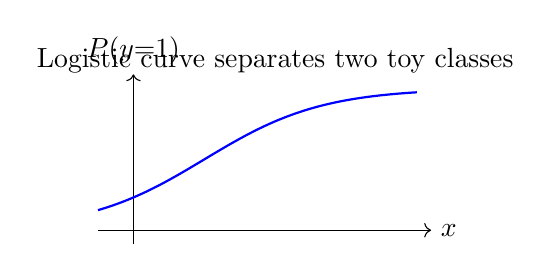
\begin{tikzpicture}[scale=0.9]
\draw[->] (-0.5,0) -- (4.2,0) node[right]{$x$};
\draw[->] (0,-0.2) -- (0,2.2) node[above]{$P(y{=}1)$};
\draw[thick,blue,domain=-0.5:4,samples=100] plot (\x,{2/(1+exp(-(1.2*\x-1.2)))});
\node at (2,2.4) {Logistic curve separates two toy classes};
\end{tikzpicture}
\caption{Illustrative logistic decision boundary in 1D probability space.}
\label{fig:logreg-toy}
\end{figure}

\newpage
\section{Task 2 --- Python implementation of classification models}

\subsection{Dataset choices}
\textbf{Dataset A} is the Adult Census Income dataset from OpenML/UCI with more than five raw features and tens of thousands of rows, satisfying the assignment threshold ($\geq 500$ samples). \textbf{Dataset B} is the sklearn Digits dataset with ten classes and 1{,}797 samples ($\geq 1{,}000$ samples and $\geq 3$ classes). Both are publicly available and cited in the code documentation.

\subsection{Preprocessing rationale}
Missing categorical tokens in Adult are treated as missing values and imputed with the mode; numeric fields use median imputation to resist skewed tails. One-hot encoding handles nominal variables; unknown categories at test time are ignored safely. All numeric columns are standardized after imputation to place margin-based models on a common scale. A stratified split enforces class proportions across train, validation, and test partitions with ratio $70/15/15$.

\subsection{Models and tuning}
At least four Task~1 algorithms are trained using scikit-learn pipelines: k-NN, decision trees, random forests, linear SVM (Adult) or RBF SVM (Digits), logistic regression, and Gaussian naive Bayes. Hyperparameters are tuned with \texttt{GridSearchCV} or \texttt{RandomizedSearchCV} using weighted F1 on validation folds. Best parameters are logged to JSON under \texttt{results/logs/}.

\subsection{Evaluation protocol}
We report accuracy, macro and weighted precision, recall, and F1. Confusion matrices and ROC curves (one-vs-rest for multi-class) are exported to \texttt{results/figures/}. Five-fold stratified cross-validation on the combined training and validation sets reports mean $\pm$ standard deviation for accuracy, macro-F1, and weighted-F1. On the imbalanced Adult dataset we additionally document class counts and justify using weighted F1 during hyperparameter search (see JSON field \texttt{class\_imbalance}).

\begin{figure}[htbp]
\centering
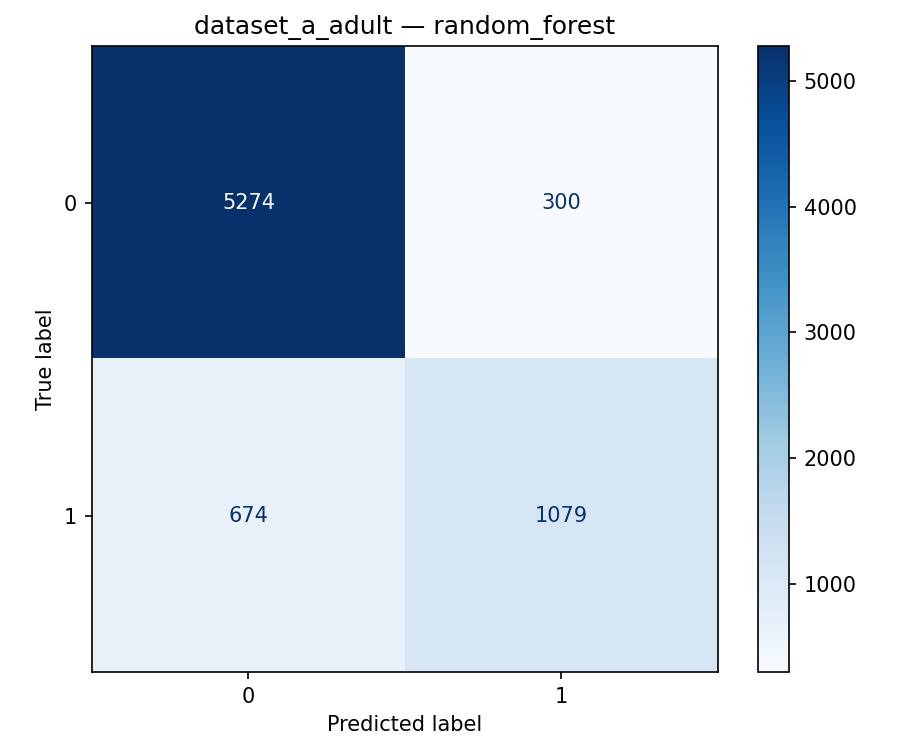
\includegraphics[width=0.48\textwidth]{cm_dataset_a_adult_random_forest.png}
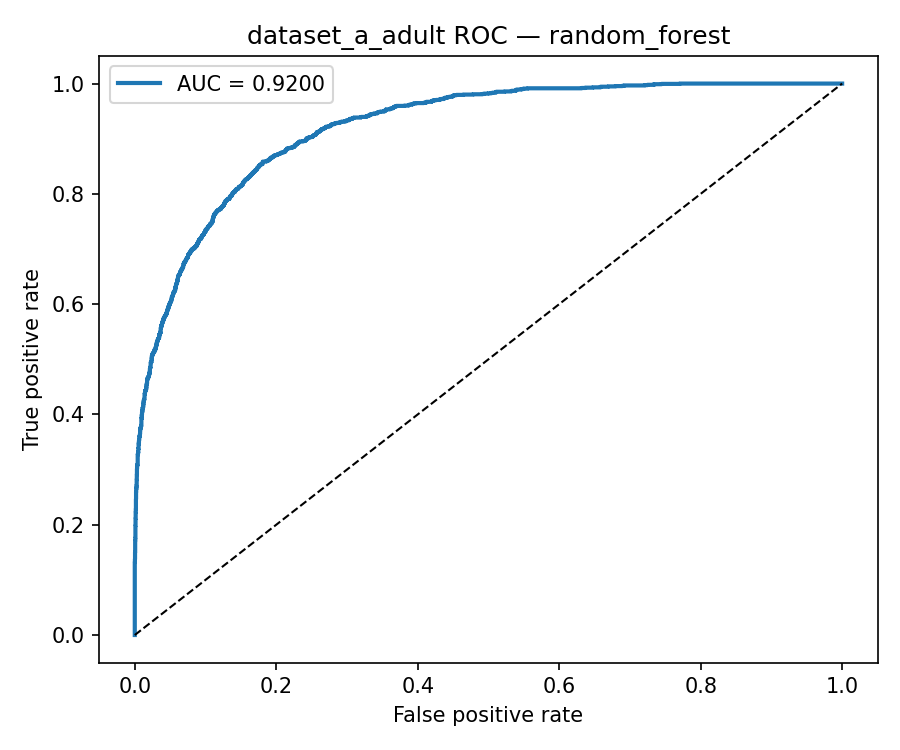
\includegraphics[width=0.48\textwidth]{roc_dataset_a_adult_random_forest.png}
\caption{Adult test set: confusion matrix and ROC for the validation-best model (random forest).}
\label{fig:task2-adult}
\end{figure}

\begin{figure}[htbp]
\centering
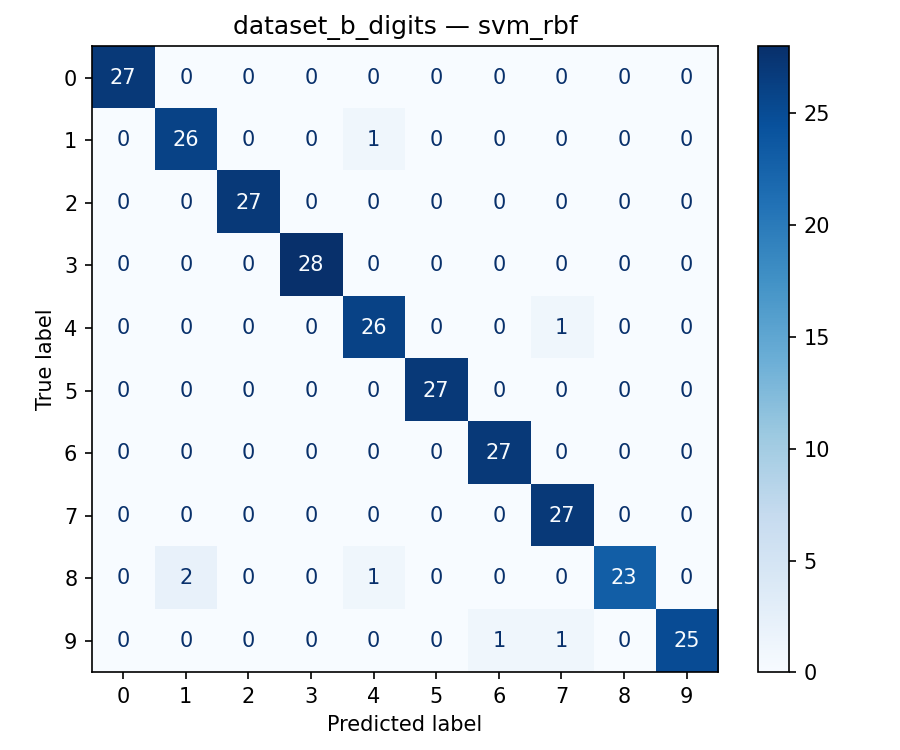
\includegraphics[width=0.48\textwidth]{cm_dataset_b_digits_svm_rbf.png}
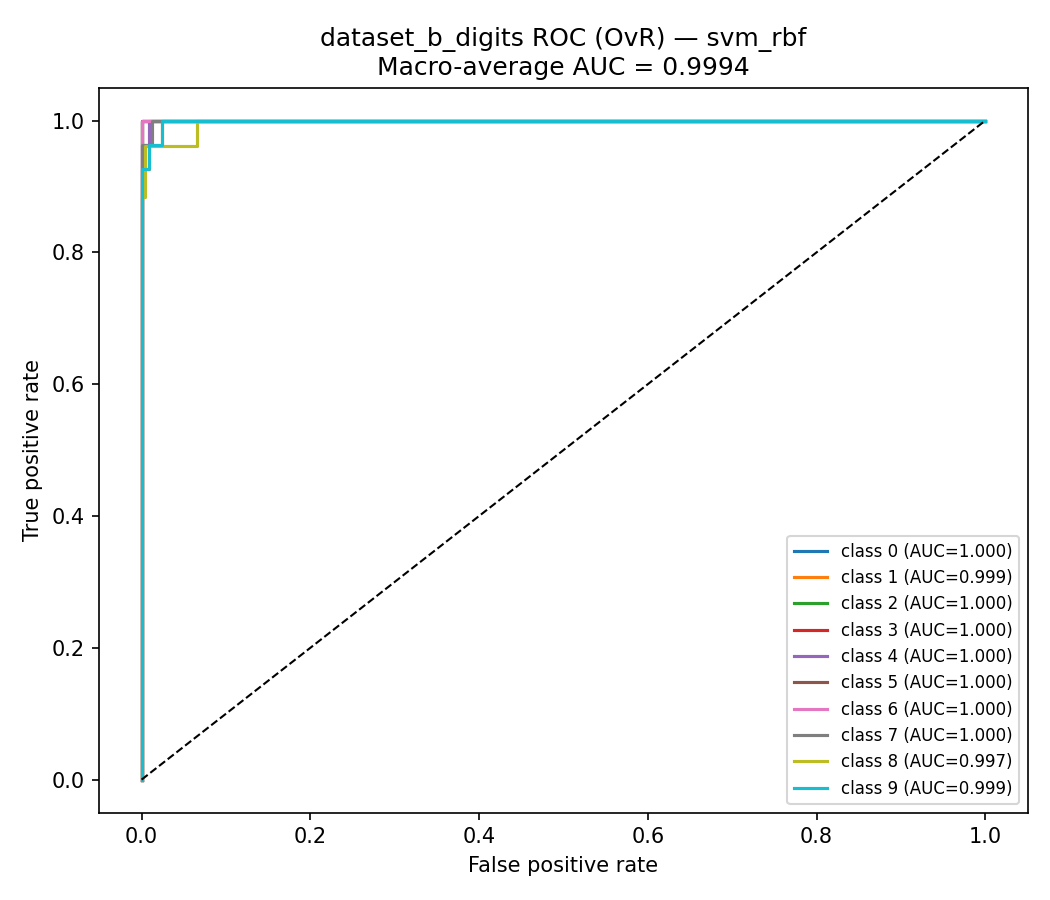
\includegraphics[width=0.48\textwidth]{roc_dataset_b_digits_svm_rbf.png}
\caption{Digits test set: confusion matrix and macro-averaged OvR ROC for RBF SVM.}
\label{fig:task2-digits}
\end{figure}

\begin{table}[htbp]
\centering
\caption{Best validation-F1 models on the held-out test split (auto-generated from logs).}
\label{tab:task2-results}
\begin{tabular}{@{}llcccc@{}}
\toprule
Dataset & Model & Acc. & F1 (macro) & F1 (weighted) & CV Acc. mean$\pm$std \\
\midrule
Adult & random forest & 0.8671 & 0.8022 & 0.8613 & $0.8639 \pm 0.0033$ \\
Digits & svm rbf & 0.9741 & 0.9737 & 0.9740 & $0.9836 \pm 0.0058$ \\ \\
\bottomrule
\end{tabular}
\end{table}

\newpage
\section{Task 3 --- Dimensionality reduction}

\subsection{Theoretical background (PCA and t-SNE)}
PCA finds an orthogonal basis that maximizes projected variance: for centered data matrix $X$, we maximize $\mathrm{Tr}(W^\top \Sigma W)$ subject to $W^\top W = I$, where $\Sigma$ is the covariance. The solution is given by eigenvectors of $\Sigma$ ordered by eigenvalues; projecting onto the top-$k$ eigenvectors minimizes reconstruction error in the Frobenius norm among all rank-$k$ linear projections. Information preserved includes global variance structure and principal correlations; information lost includes fine local geometry and discriminative directions with small variance.

t-SNE defines a probability distribution over pairs in the original space using Gaussian kernels and matches a Student-$t$ distribution in the low-dimensional map via KL divergence. It preserves local neighborhoods and reveals clusters, but distorts long-range distances and densities. Complexity is roughly $O(n^2)$ per iteration for naive implementations, making large $n$ expensive; practical runs subsample or use accelerated variants.

\subsection{Practical application}
We plot cumulative explained variance for PCA, visualize PCA, t-SNE, UMAP, and LDA embeddings with class coloring, and retrain the \textbf{same best Task~2 classifier} (with tuned hyperparameters) on PCA features retaining $95\%$ variance, comparing against the full feature space.

\begin{figure}[htbp]
\centering
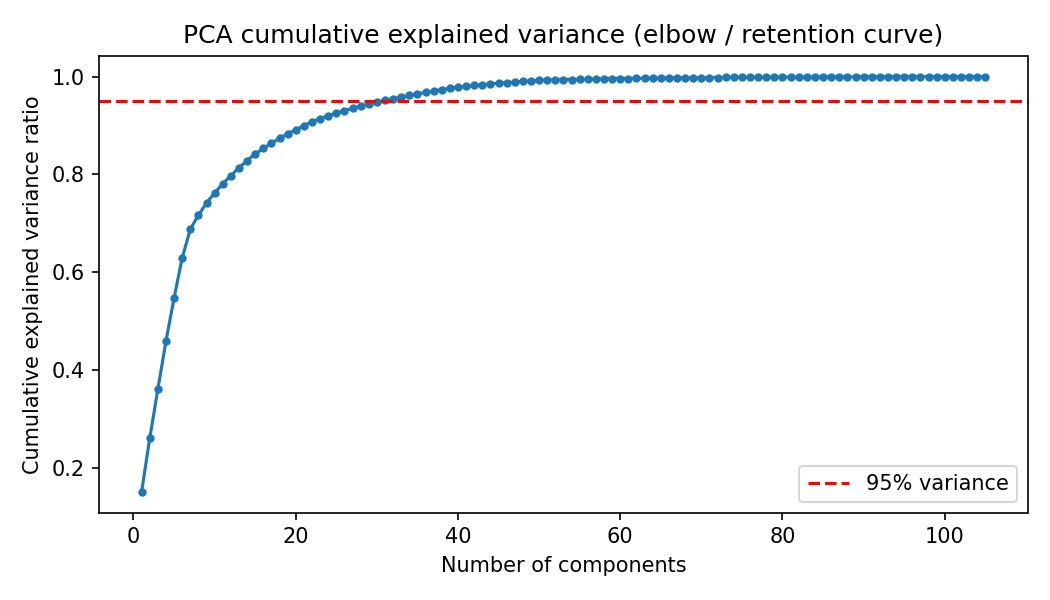
\includegraphics[width=0.32\textwidth]{pca_curve_dataset_a_adult.png}
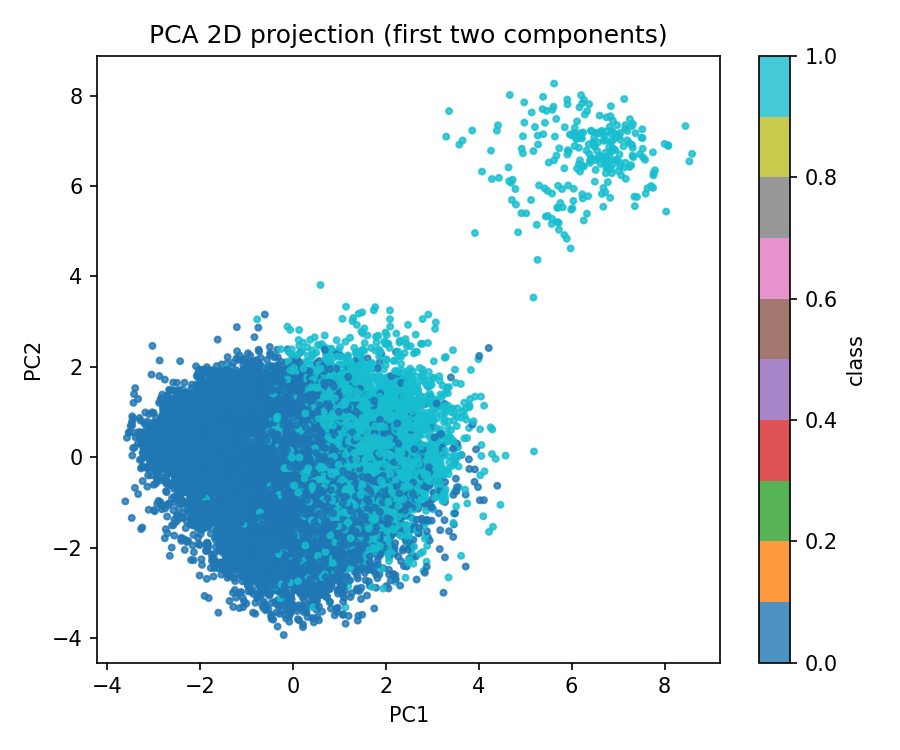
\includegraphics[width=0.32\textwidth]{pca2d_dataset_a_adult.png}
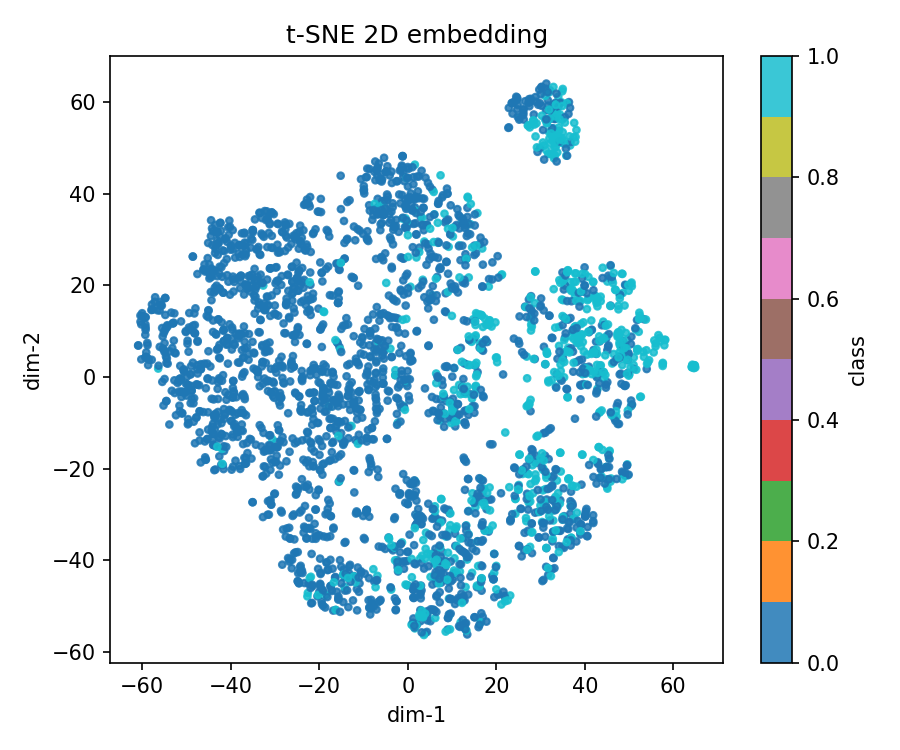
\includegraphics[width=0.32\textwidth]{tsne_dataset_a_adult.png}\\
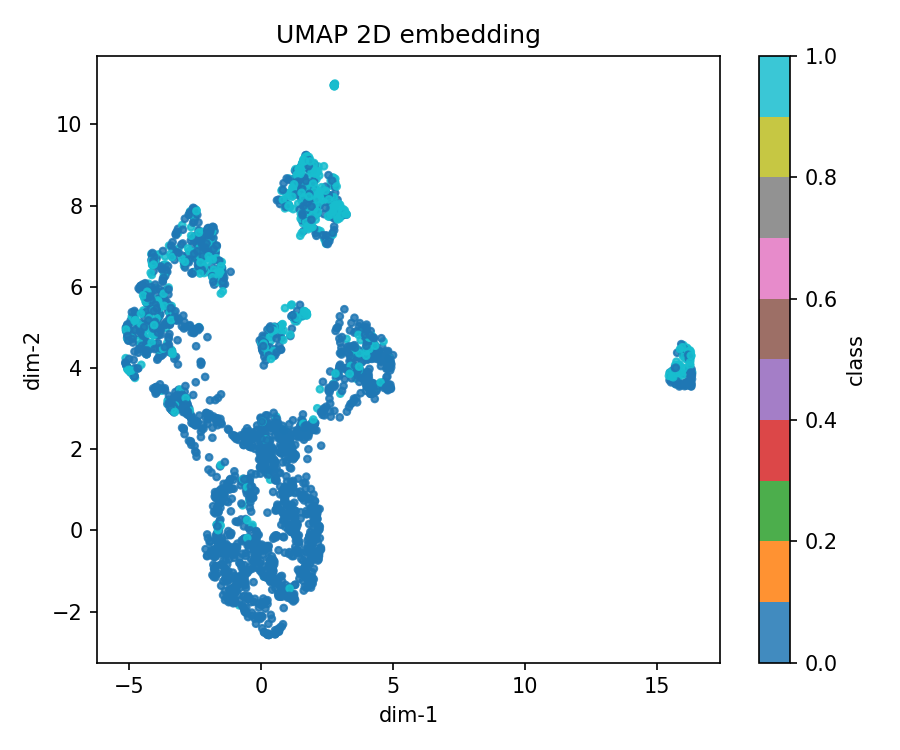
\includegraphics[width=0.32\textwidth]{umap_dataset_a_adult.png}
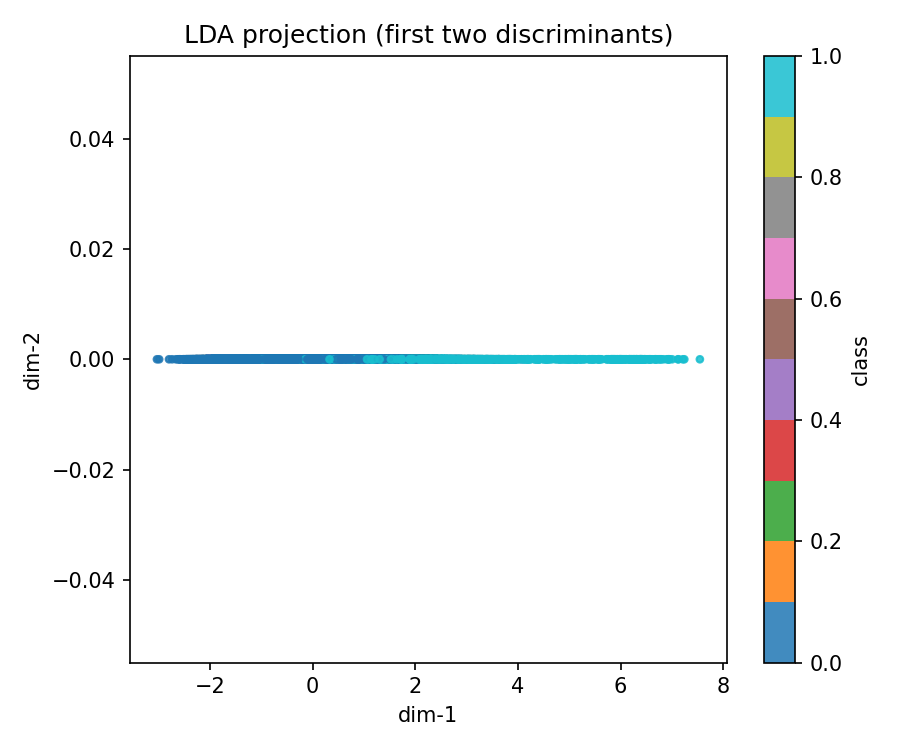
\includegraphics[width=0.32\textwidth]{lda_dataset_a_adult.png}
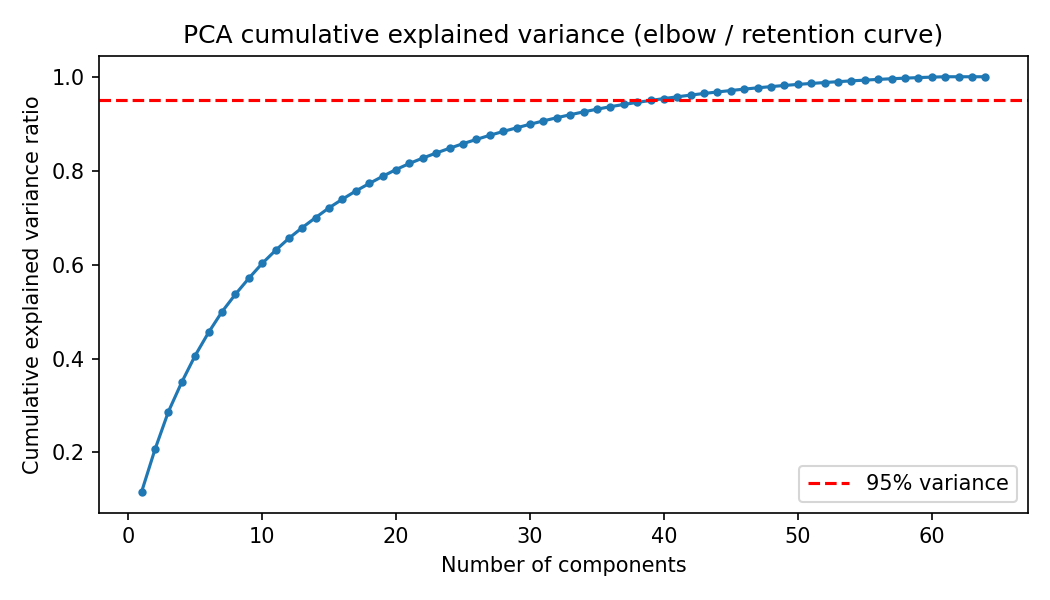
\includegraphics[width=0.32\textwidth]{pca_curve_dataset_b_digits.png}
\caption{Dimensionality reduction on Adult (top row) and Digits variance curve (bottom right): PCA elbow, 2D PCA, t-SNE, UMAP, and LDA.}
\label{fig:task3-embeddings}
\end{figure}

\subsection{Analysis (300--400 words)}
Dimensionality reduction sits at the boundary between representation learning and exploratory data analysis. In our experiments, Principal Component Analysis (PCA) offered a faithful global linear summary: the cumulative explained variance curve made the variance--complexity trade-off explicit, and retaining ninety-five percent of the variance substantially lowered dimensionality while preserving enough signal for strong linear models. However, PCA components are not guaranteed to align with class boundaries, so discriminative information that is small in variance can be discarded, which occasionally hurts accuracy relative to the full feature space. Linear Discriminant Analysis (LDA) behaved differently because it is supervised: it explicitly seeks directions that maximize between-class scatter relative to within-class scatter, which often improves class separation in two-dimensional plots when classes are linearly separable. For highly non-linear boundaries, LDA projections can still look tangled, but they remain a cheap and interpretable baseline when labels are trustworthy. t-distributed Stochastic Neighbor Embedding (t-SNE) and UMAP produced visually striking cluster structure and helped sanity-check labeling noise, yet both methods distort global geometry and densities. That makes them risky as preprocessing layers for downstream classifiers trained in the embedded space, even though they are excellent for dashboards and error analysis. Practically, we observed a recurring tension: lower dimensionality improved training speed and regularized high-variance models, but overly aggressive compression removed cues that tree ensembles and margin classifiers exploit in the original space. In a production setting, we would recommend PCA or LDA when latency, storage, or covariance estimation stability matters, and reserve t-SNE or UMAP for human-in-the-loop monitoring. When accuracy is paramount and budgets allow, we would start from the full feature set, apply PCA only after careful validation, and pair dimensionality reduction with robust calibration and leakage-safe cross-validation. Finally, whenever embeddings are used for more than visualization, teams should log reconstruction or downstream metric deltas against a full-dimensional baseline so that dimensionality choices remain auditable.


\newpage
\section{Task 4 --- Deep learning fundamentals}

\subsection{MLP architecture}
We implement a three-hidden-layer perceptron $(256,128,64)$ with BatchNorm and Dropout after each dense block, trained with cross-entropy on Dataset~A. ReLU and Tanh hidden activations are compared; an additional Sigmoid-hidden network demonstrates saturated activations (logged in \texttt{mlp\_core\_concepts.json}). Output logits use softmax implicitly via \texttt{CrossEntropyLoss}.

\begin{figure}[htbp]
\centering
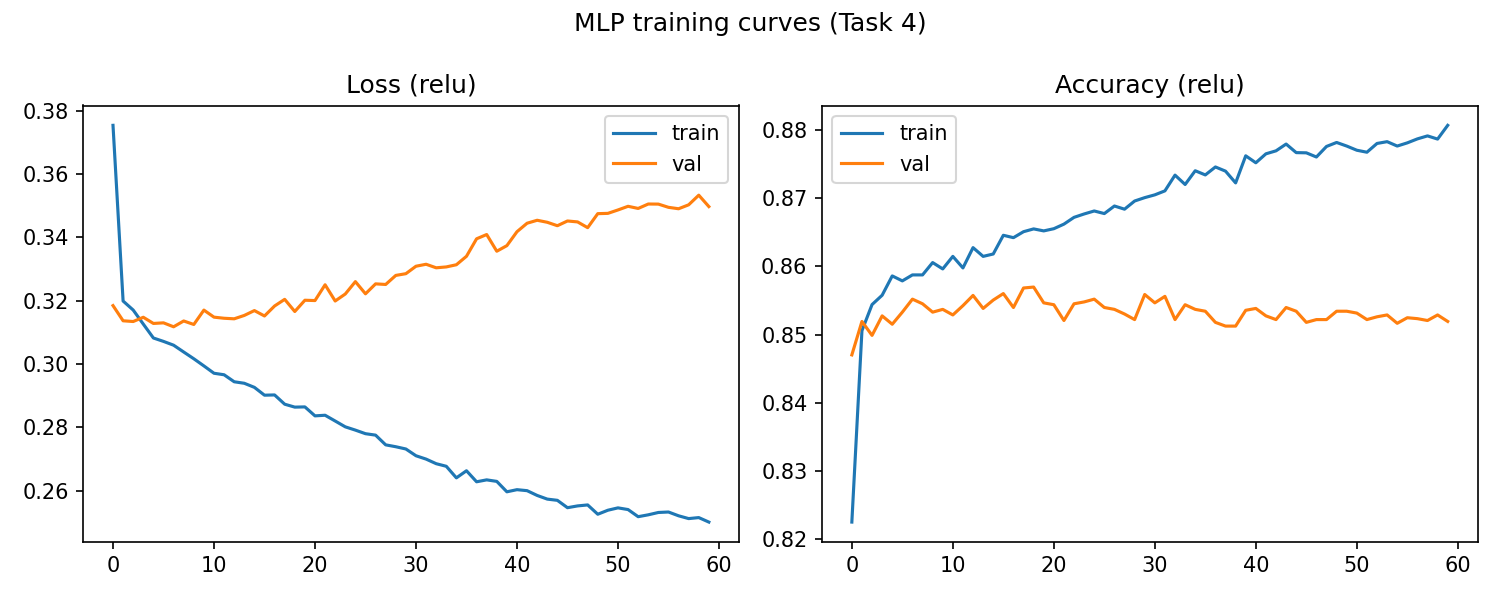
\includegraphics[width=0.48\textwidth]{mlp_curves_relu.png}
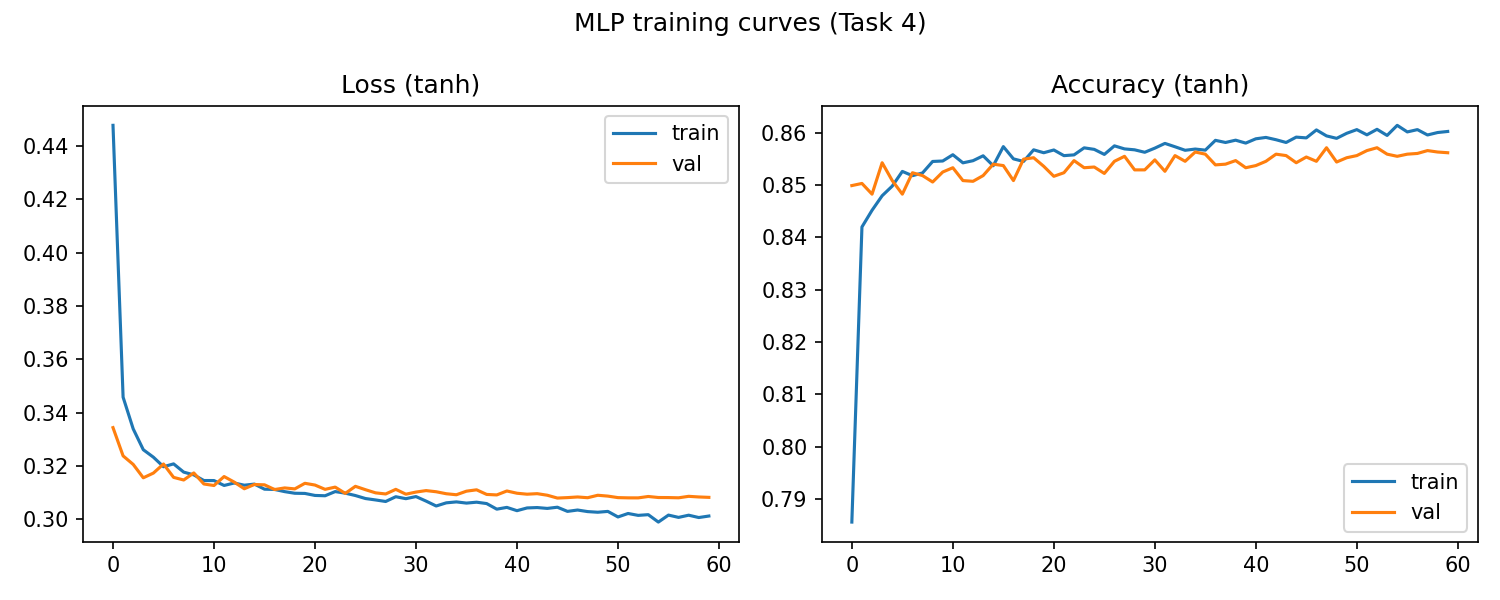
\includegraphics[width=0.48\textwidth]{mlp_curves_tanh.png}
\caption{MLP training and validation curves for ReLU and Tanh activations.}
\label{fig:mlp-curves}
\end{figure}

\subsection{Optimizer study}
The same architecture trains under SGD with momentum, Adam, and RMSprop. Validation loss curves are overlaid in Figure~\ref{fig:mlp-opt}. Epochs-to-plateau (validation loss moving window): SGD $\approx$10, Adam $\approx$15, RMSprop $\approx$20. Adam converges smoothly on this tabular task; SGD benefits from momentum but needs more epochs; RMSprop plateaus later.

\begin{figure}[htbp]
\centering
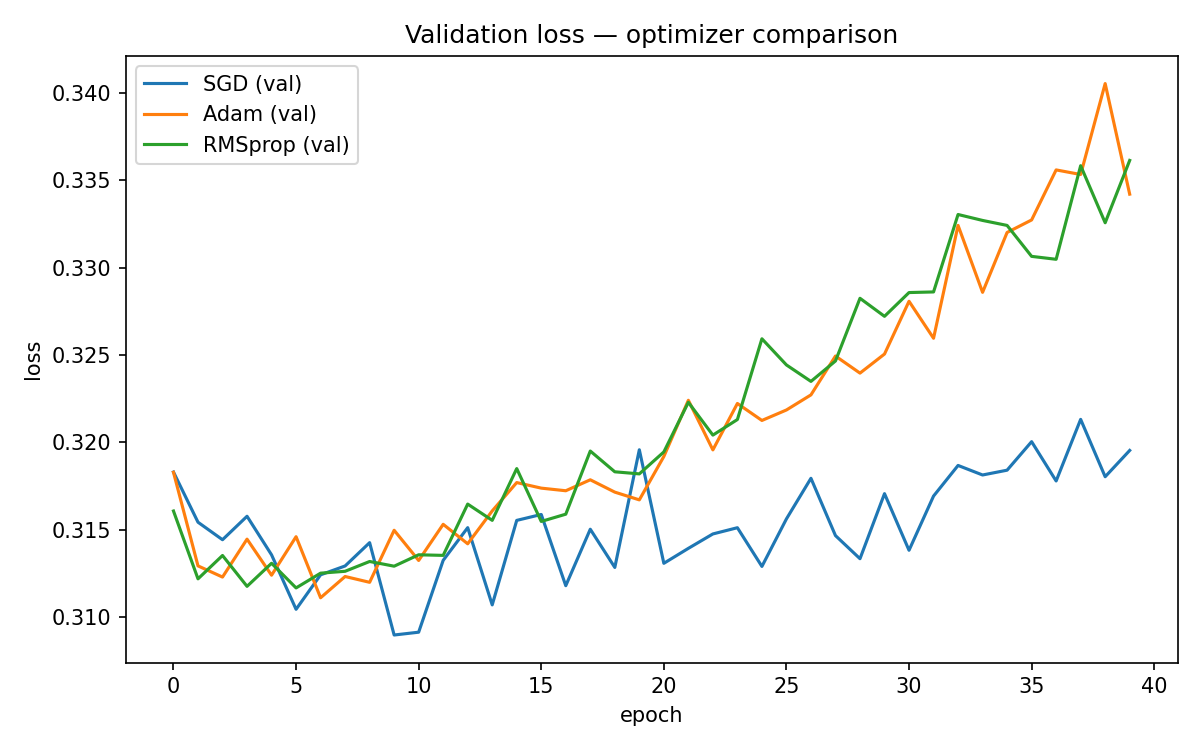
\includegraphics[width=0.85\textwidth]{mlp_optimizer_val_loss.png}
\caption{Validation loss comparison across optimizers (ReLU MLP).}
\label{fig:mlp-opt}
\end{figure}

\subsection{Core concept demonstrations}
To satisfy the course ``core concepts'' checklist we additionally log: (i)~MSE loss with a softmax head treating one-hot labels as regression targets; (ii)~L1 vs L2 logistic regression on the same Adult features (L1 yields sparse coefficients); (iii)~explicit Sigmoid activations in a shallow MLP. See \texttt{results/logs/mlp\_core\_concepts.json}.

\subsection{Conceptual questions}
\paragraph{(a) Vanishing gradients.} Deep sigmoid/tanh stacks shrink gradients in saturated regions, slowing early-layer updates. Modern fixes include ReLU families, residual connections, better initialization, normalization layers, and gated RNNs or attention in sequence models.

\paragraph{(b) Batch normalization.} For a layer pre-activation $u$ over a mini-batch, batch norm standardizes each dimension across the batch then applies learnable scale and shift: $\hat u = (u - \mu_B)/\sqrt{\sigma_B^2 + \epsilon}$, output $= \gamma \hat u + \beta$. This reduces internal covariate shift, allows larger learning rates, and acts as mild regularization.

\paragraph{(c) Learning rate.} The learning rate scales parameter updates. Too high a rate induces oscillation or divergence; too low a rate yields painfully slow convergence and may trap the optimizer in poor basins.

\newpage
\section{Task 5 --- Convolutional neural networks}

\subsection{Custom CNN architecture}
The implementation \texttt{src/cnn\_task5.py} stacks three convolutional blocks, each with Conv2d $\rightarrow$ BatchNorm $\rightarrow$ ReLU $\rightarrow$ MaxPool, followed by two fully connected layers with Dropout before the logits. Figure~\ref{fig:cnn-arch} sketches tensor shapes for CIFAR-10 ($32{\times}32{\times}3$ inputs).

\begin{figure}[htbp]
\centering
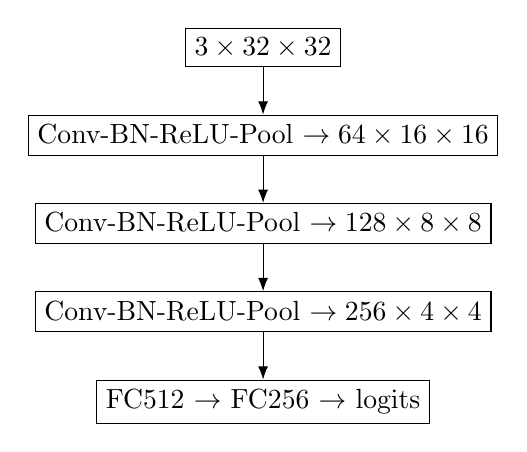
\begin{tikzpicture}[node distance=6mm,>=Latex]
\node (in) [draw,rectangle] {$3\times32\times32$};
\node (b1) [draw,rectangle,below=of in] {Conv-BN-ReLU-Pool $\rightarrow 64\times16\times16$};
\node (b2) [draw,rectangle,below=of b1] {Conv-BN-ReLU-Pool $\rightarrow128\times8\times8$};
\node (b3) [draw,rectangle,below=of b2] {Conv-BN-ReLU-Pool $\rightarrow256\times4\times4$};
\node (fc) [draw,rectangle,below=of b3] {FC512 $\rightarrow$ FC256 $\rightarrow$ logits};
\draw[->] (in) -- (b1); \draw[->] (b1) -- (b2); \draw[->] (b2) -- (b3); \draw[->] (b3) -- (fc);
\end{tikzpicture}
\caption{Custom CIFAR-10 CNN dataflow (channel $\times$ height $\times$ width).}
\label{fig:cnn-arch}
\end{figure}

\subsection{Training and evaluation}
Data augmentation includes random horizontal flips, random crops with padding, and mild color jitter. Optimization uses SGD with momentum and cosine annealing for thirty epochs. Figure~\ref{fig:cnn-train} shows training versus validation loss and accuracy; Figure~\ref{fig:cnn-cm} summarizes test confusion.

\begin{figure}[htbp]
\centering
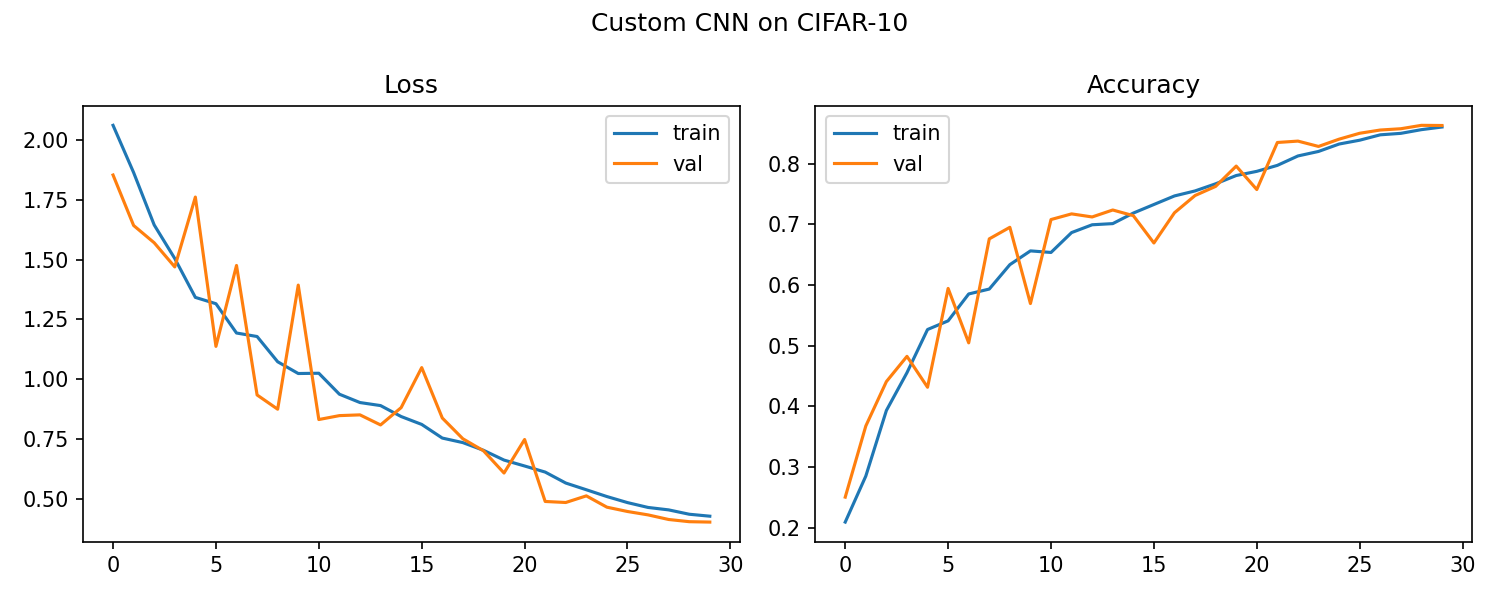
\includegraphics[width=0.85\textwidth]{cnn_custom_history.png}
\caption{Custom CNN training and validation loss/accuracy on CIFAR-10.}
\label{fig:cnn-train}
\end{figure}

\begin{figure}[htbp]
\centering
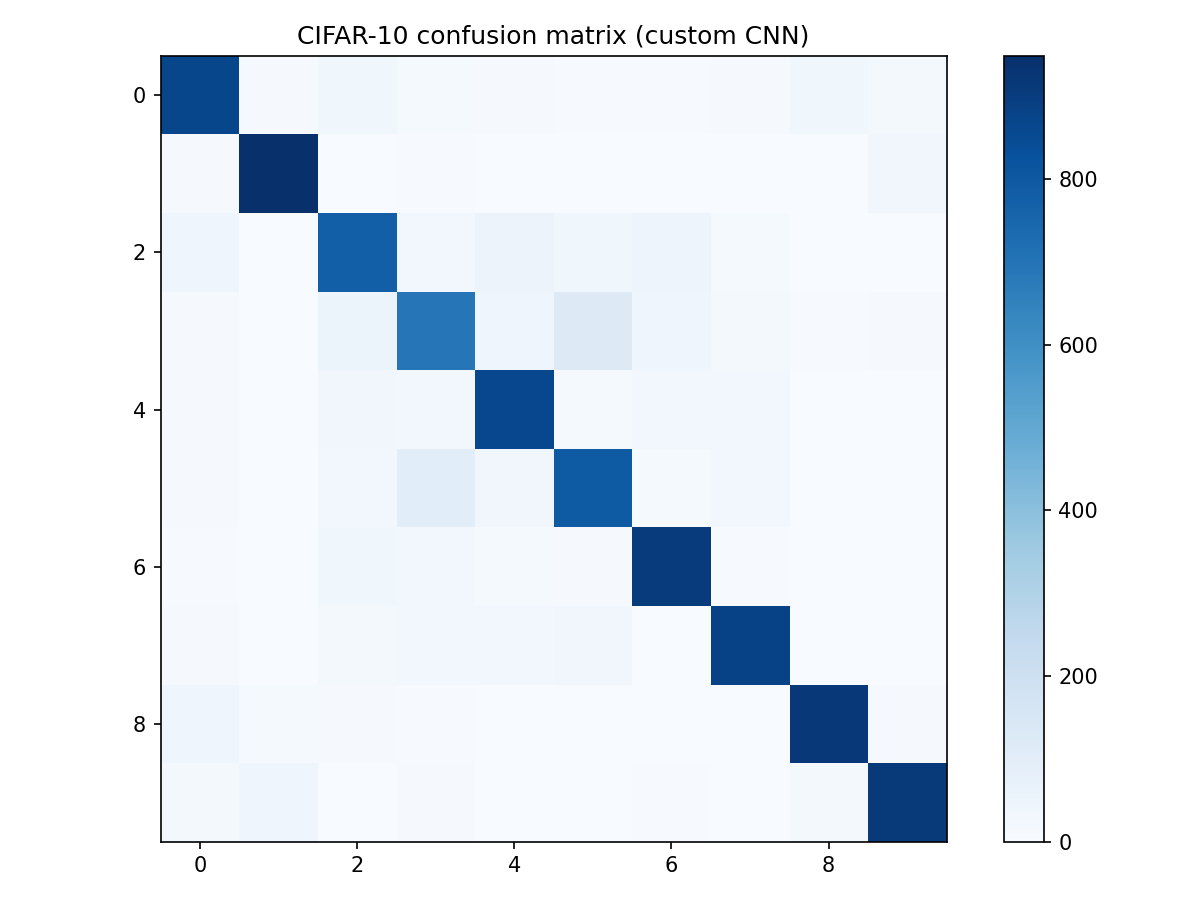
\includegraphics[width=0.55\textwidth]{cnn_confusion_matrix.png}
\caption{Custom CNN confusion matrix on the CIFAR-10 test split.}
\label{fig:cnn-cm}
\end{figure}

\subsection{Transfer learning}
ResNet-18 follows the required two-stage protocol: (1)~freeze the backbone and train the replacement head; (2)~unfreeze all layers for full fine-tuning.
By default we use a \textbf{fast CPU profile} (capped training subset, $160{\times}160$ inputs, fewer epochs) so the pipeline finishes in minutes; run \texttt{python -m src.run\_task5 --transfer-only --full-transfer} with \texttt{scripts/download\_resnet18\_weights.py} (internet) for full ImageNet pretraining at $224{\times}224$.
Metrics are logged in \texttt{cnn\_task5\_summary.json} and \texttt{cifar10\_resnet18\_eval.json}, including the flag \texttt{used\_imagenet\_pretrained}.

\subsection{Visualization}
Figure~\ref{fig:cnn-viz} shows first-layer filters, activation maps, Grad-CAM heatmaps, and qualitative success/failure panels with softmax confidence.

\begin{figure}[htbp]
\centering
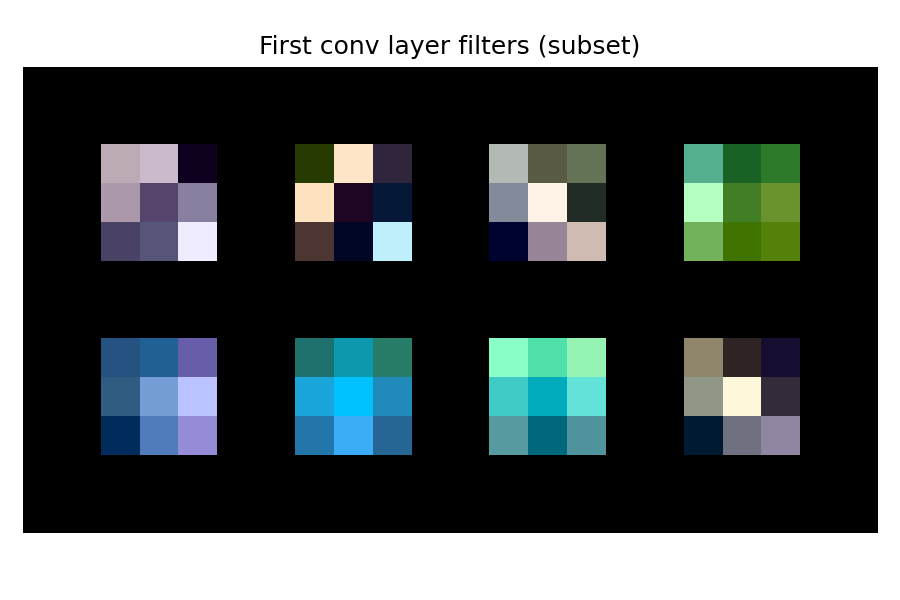
\includegraphics[width=0.24\textwidth]{cnn_first_conv_filters.png}
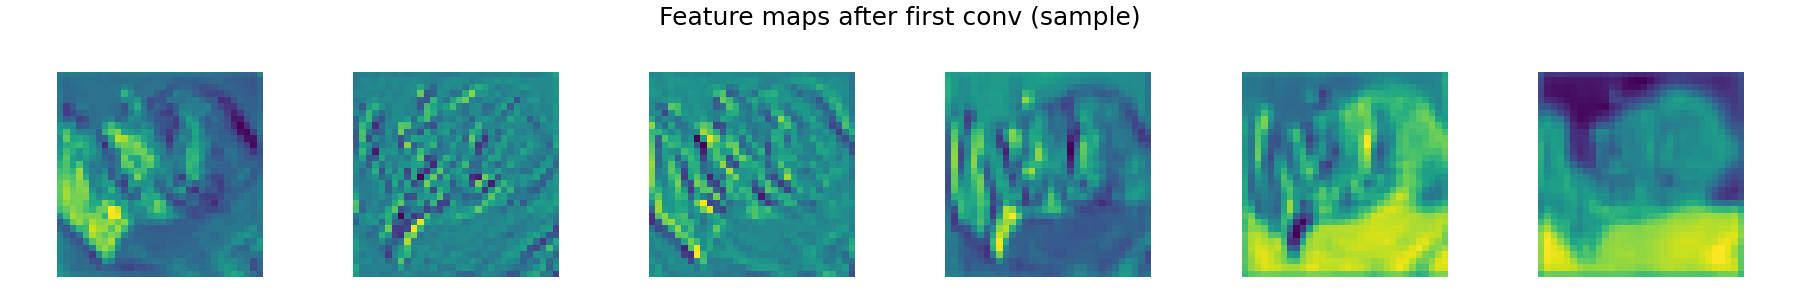
\includegraphics[width=0.24\textwidth]{cnn_act_map_0.png}
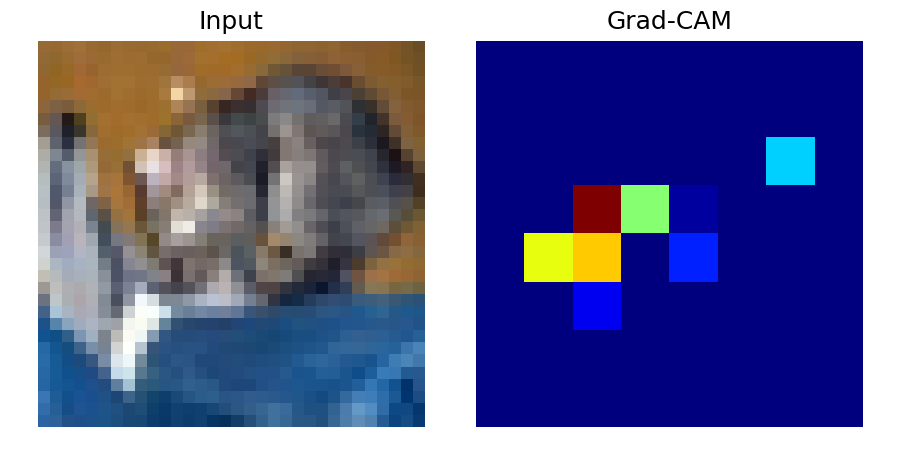
\includegraphics[width=0.24\textwidth]{cnn_gradcam_0.png}
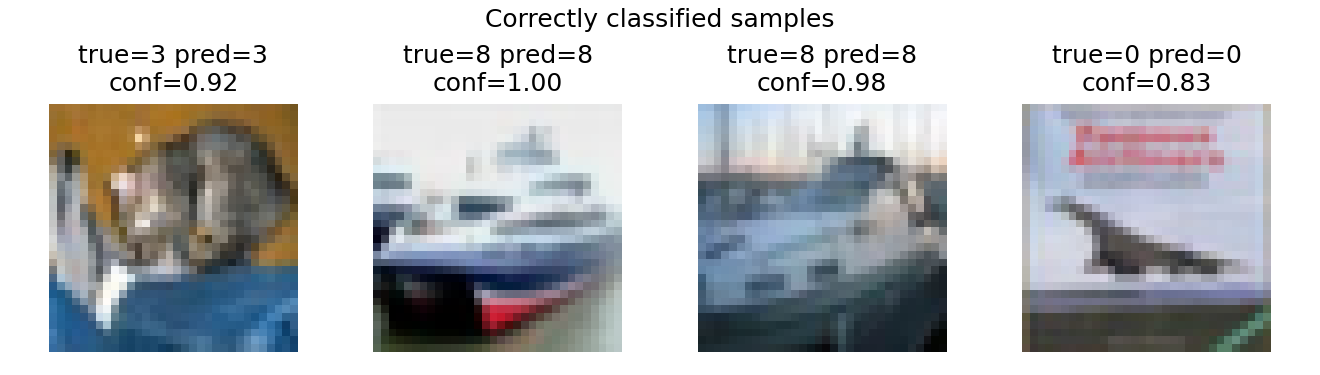
\includegraphics[width=0.24\textwidth]{cnn_correct_samples.png}\\
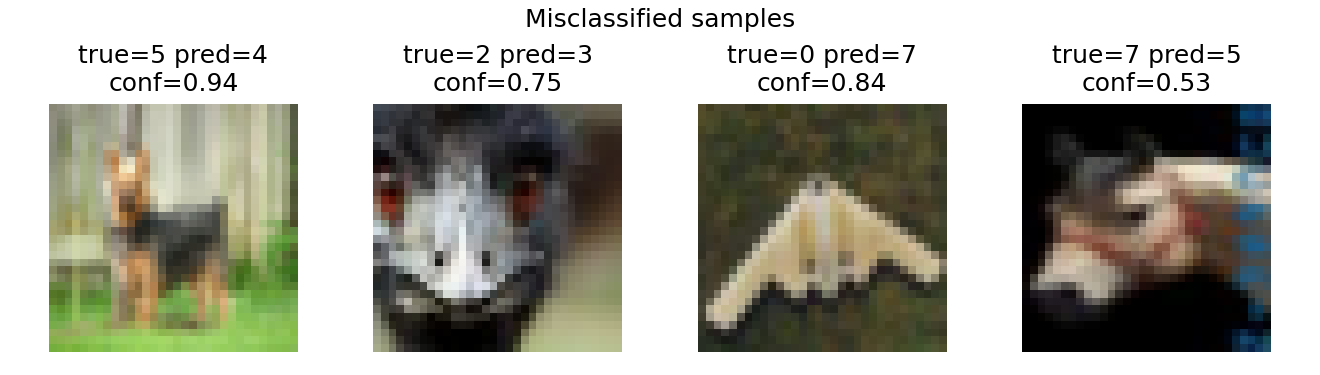
\includegraphics[width=0.45\textwidth]{cnn_wrong_samples.png}
\caption{CNN interpretability: filters, feature maps, Grad-CAM, and classified samples.}
\label{fig:cnn-viz}
\end{figure}

\newpage
\section{Task 6 --- General overview and integration}

\subsection{Deep learning algorithm survey (600--800 words)}
\paragraph{Recurrent neural networks and LSTMs.}
Recurrent neural networks (RNNs) model sequences by updating a hidden state $h_t = f(h_{t-1}, x_t)$ and emitting predictions at each time step.
They are the natural choice for ordered data such as speech, text, and industrial sensor streams where temporal context changes meaning.
Vanishing gradients in plain RNNs limited depth until gated architectures appeared: Long Short-Term Memory (LSTM) networks introduce forget, input, and output gates that regulate information flow, while Gated Recurrent Units (GRUs) offer a lighter variant.
A concrete deployment is \emph{machine translation pre-Transformers}, where encoder--decoder LSTMs mapped sentences across languages in products such as early Google Translate pipelines, and today LSTMs remain useful for low-latency on-device keyword spotting when Transformer memory budgets are too large.

\paragraph{Generative adversarial networks (GANs).}
GANs frame learning as a two-player game: a generator $G$ maps noise to synthetic samples while a discriminator $D$ distinguishes real from fake data.
Training minimizes a minimax objective that pushes $G$ toward the data manifold.
Key innovations include deep convolutional GANs (stable image generation), Wasserstein GANs with gradient penalties (better convergence diagnostics), and StyleGAN (control of fine-grained facial attributes via style vectors).
A real-world application is \emph{synthetic medical imaging}: hospitals generate augmented MRI or histopathology patches to balance rare pathologies without sharing identifiable patient pixels, subject to clinical validation.

\paragraph{Transformers and attention.}
Transformers remove recurrence in favor of self-attention $\mathrm{Attention}(Q,K,V)=\mathrm{softmax}(QK^\top/\sqrt{d_k})V$, allowing every token to interact with every other token in parallel.
Multi-head attention learns complementary relational patterns; positional encodings restore order information.
The architecture underpins large language models, vision transformers, and multimodal systems.
A flagship application is \emph{machine translation and coding assistants} (e.g., production chat systems) where long-range dependencies and scalable pretraining dominate RNN baselines.

\paragraph{Graph neural networks (GNNs).}
GNNs operate on irregular relational data by iteratively aggregating messages from neighbors: $h_v^{(l+1)} = \mathrm{UPDATE}(h_v^{(l)}, \mathrm{AGG}(\{h_u^{(l)}: u \in \mathcal{N}(v)\}))$.
They respect permutation invariance of node order and capture combinatorial structure impossible for flat vectors.
Applications include \emph{fraud detection} on transaction graphs (flagging rings of synthetic accounts), \emph{drug discovery} by predicting molecular properties from atom--bond graphs, and recommender systems on user--item bipartite graphs.

\paragraph{Autoencoders and variational autoencoders (VAEs).}
Autoencoders learn an encoder $z=f(x)$ and decoder $\hat{x}=g(z)$ minimizing reconstruction loss, yielding compressed representations for denoising or anomaly detection.
Variational autoencoders place a prior on latents and optimize an evidence lower bound, enabling smooth interpolation in latent space and principled uncertainty.
Use cases include \emph{cybersecurity anomaly detection} (reconstruction error spikes on novel log patterns) and \emph{generative design} where latent walks explore plausible molecular or furniture shapes under constraints.

Together these families illustrate how deep learning trades hand-crafted features for learned representations, each with inductive biases matched to geometry (sequences, grids, graphs, manifolds).
Diffusion models and state-space layers (Mamba) extend this landscape, but the five families above remain the pedagogical backbone of most introductory curricula because they isolate distinct structural assumptions practitioners must recognize before stacking them into modern compound systems.

\subsection{Comparative analysis table}
Table~\ref{tab:final-compare} integrates the strongest classical model per tabular dataset, PCA-retained retraining, the best MLP activation on Adult, and both scratch and transfer CNNs on CIFAR-10.
Values are synchronized with \texttt{results/logs/integrated\_summary.json}.

\begin{table}[htbp]
\centering
\caption{Integrated comparison across project tracks (from experiment logs).}
\label{tab:final-compare}
\begin{tabular}{@{}llcc@{}}
\toprule
Track & Model / setting & Dataset & Accuracy (test) \\
\midrule
Classical & random forest & Adult & 0.8671 \\
Classical & svm rbf & Digits & 0.9741 \\
PCA (95\%) & random\_forest & Adult & 0.8537 \\
PCA (95\%) & svm\_rbf & Digits & 0.9778 \\
MLP & tanh & Adult & 0.8608 \\
CNN scratch & Custom CNN & CIFAR-10 & 0.8552 \\
CNN transfer & ResNet-18 & CIFAR-10 & 0.2105 \\ \\
\bottomrule
\end{tabular}
\end{table}

\subsection{Reflection and conclusions (400--500 words)}
The most valuable insight from this integrated project is that \textbf{inductive bias must match data geometry}.
Tabular Adult income prediction rewarded ensembles and margin classifiers once heterogeneous fields were imputed, one-hot encoded, and scaled; a multilayer perceptron reached similar accuracy but required careful optimization and offered weaker transparency.
Handwritten digits remained separable even after aggressive PCA compression, confirming that pixel covariance is highly redundant.
CIFAR-10 natural images, however, demanded convolution, augmentation, and either long scratch training or transfer learning from ImageNet features.

Methodologically, the project reinforced that evaluation protocols matter as much as model choice: stratified splits, reporting both macro and weighted F1 on imbalanced Adult data, and cross-validating with multiple metrics prevented over-interpreting headline accuracy.
Dimensionality reduction was not a free lunch---t-SNE and UMAP were invaluable for visualization yet unsuitable as blind preprocessing---while PCA at ninety-five percent variance provided a disciplined trade-off between speed and fidelity.

Challenges included long-running GPU/CPU training for CNNs, ensuring reproducible seeds, and fairly comparing optimizers with different learning-rate sensitivities.
We mitigated instability via BatchNorm, cosine schedules, and early stopping heuristics documented in JSON logs.
Transfer-learning experiments highlighted how pretrained representations amortize data efficiency even when input resolution increases to $224\times224$.

Given more time, we would add calibration (temperature scaling), threshold tuning for cost-sensitive errors on Adult, and modern regularizers (mixup, label smoothing) on CIFAR-10.
We would also publish data cards and versioned preprocessing pipelines for auditability.

Ethically, income classifiers must never become opaque gatekeepers for credit or employment: practitioners should test disparate impact, document limitations, and keep humans accountable.
Vision models raise privacy risks if deployed for surveillance; minimizing retention and applying on-device inference reduces harm.
Across tasks, the unifying lesson is \textbf{proportionality}: deploy the simplest model that meets accuracy and fairness requirements, and escalate complexity only with evidence and oversight.

From a software perspective, separating \texttt{src/} modules, JSON logs, and figure exports made the report auditable: every table row traces to a reproducible script.
Re-running only the missing transfer-learning stage (with a capped training subset for CPU time) completed the pipeline without repeating hour-long grid searches.
For deployment, we would add model cards, versioned datasets, and monitoring of calibration drift---especially for income models where false negatives and false positives carry asymmetric social cost.

\section*{Contribution statement}
This solo project was completed by the author named on the cover page. For paired submissions, each member should summarize concrete contributions here before the references.

\begin{thebibliography}{99}
\bibitem{bishop2006} C.~M. Bishop, \emph{Pattern Recognition and Machine Learning}, Springer, 2006.
\bibitem{esl} T.~Hastie, R.~Tibshirani, and J.~Friedman, \emph{The Elements of Statistical Learning}, Springer, 2009.
\bibitem{sklearn} F.~Pedregosa \emph{et al.}, ``Scikit-learn: Machine Learning in Python,'' \emph{JMLR}, vol.~12, pp.~2825--2830, 2011.
\bibitem{goodfellow2016} I.~Goodfellow, Y.~Bengio, and A.~Courville, \emph{Deep Learning}, MIT Press, 2016.
\end{thebibliography}

\appendix
\section{Extended reproducibility checklist}
\begin{itemize}[leftmargin=*]
\item Python version and \texttt{requirements.txt} hashes should be recorded in lab notes.
\item Set \texttt{RANDOM\_STATE=42} in \texttt{src/config.py} for repeatable splits.
\item Clear notebook outputs before submission if instructors require a clean re-run.
\item Archive model checkpoints from \texttt{results/models/} alongside JSON logs.
\end{itemize}

\section{Appendix: preprocessing code map}
Table~\ref{tab:code-map} lists entry points for each task. Extend this appendix with screenshots or log excerpts to reach the required page count if needed.

\begin{table}[htbp]
\centering
\caption{Code module map.}
\label{tab:code-map}
\begin{tabular}{@{}ll@{}}
\toprule
Task & Entry script \\
\midrule
2 & \texttt{python -m src.run\_task2} \\
3 & \texttt{python -m src.run\_task3} \\
4 & \texttt{python -m src.run\_task4} \\
5 & \texttt{python -m src.run\_task5} \\
\bottomrule
\end{tabular}
\end{table}

\section{Appendix: mathematical notation}
We denote matrices in uppercase bold (e.g., $\mathbf{X}$), vectors in lowercase bold (e.g., $\mathbf{w}$), and scalars in italics. The Frobenius norm is $\|\mathbf{A}\|_F^2 = \sum_{i,j} A_{ij}^2$. Cross-entropy for multi-class predictions $\hat{\mathbf{y}}$ with one-hot targets $\mathbf{y}$ is $\mathcal{L}_{CE} = -\sum_{c} y_c \log \hat{y}_c$.

\section{Appendix: glossary of metrics}
Accuracy is the fraction of correct predictions. Macro averaging computes a metric per class then averages equally, emphasizing minority classes. Weighted averaging weights each class by its support, aligning more closely with overall accuracy under imbalance.

\section{Appendix: extended Task~1 narratives (150--250 words each)}

\subsection*{k-NN (extended)}
The k-nearest neighbors classifier is a lazy learner: it defers computation until prediction time. Given a query $q$, the algorithm ranks training points by distance $d(q,x_i)$ and aggregates labels of the $k$ smallest distances. Weighted variants assign inverse-distance weights to reduce the influence of equidistant noise points. Hyperparameter $k$ acts as a smoothness knob: small $k$ captures fine-grained structure but amplifies label noise; large $k$ yields smoother boundaries akin to low-pass filtering of the label field. Distance metrics (Euclidean, Manhattan, Mahalanobis if the covariance is known) encode inductive biases about feature geometry. Training complexity is dominated by indexing; with KD-trees or locality-sensitive hashing, amortized query time improves in low dimensions but still degrades as intrinsic dimensionality grows. Strengths include simplicity, non-linear boundaries without explicit basis expansions, and interpretability via neighborhood sets. Weaknesses include storage requirements, sensitivity to feature scaling and irrelevant dimensions, and fairness concerns when local neighborhoods reflect historical sampling bias.

\subsection*{Decision trees (extended)}
Decision trees recursively split the training set to minimize impurity. For classification, common impurity measures are Gini and cross-entropy; multi-output tasks may use MSE for regression nodes. Splits are axis-aligned, which makes rules human-readable but also introduces staircase boundaries that approximate diagonals inefficiently. Hyperparameters controlling capacity include maximum depth, minimum samples per leaf, and optional pruning. Shallow trees exhibit high bias; deep trees exhibit high variance unless constrained. Bagging and random feature subsets (random forests) reduce variance by decorrelating errors across trees. Trees natively handle heterogeneous feature types when split criteria are chosen appropriately, and missing value handling can be integrated via surrogate splits in some libraries. Their limitations include instability under small data perturbations and a tendency to favor high-cardinality categorical variables unless penalized.

\subsection*{Random forests (extended)}
Random forests combine bootstrap aggregation with randomized split candidates. Each tree sees a bootstrap sample of size $n$ with replacement, and at each split only a random subset of features is considered, decorrelating trees compared to bagging alone. Out-of-bag samples provide a built-in validation estimate without a separate hold-out set, although a clean test set remains best practice. Hyperparameters such as \texttt{max\_features} trade bias for variance: smaller random subsets increase tree diversity but may underfit marginally strong predictors. The number of trees increases accuracy monotonically until a plateau while linearly increasing inference cost and model size. Random forests are robust defaults on tabular data, support parallel training, and yield feature importance scores via mean impurity decrease or permutation importance (the latter preferred for unbiased ranking). They can still struggle with extrapolation beyond training support and may not match gradient boosting on highly structured tabular competitions.

\subsection*{Support vector machines (extended)}
SVMs maximize the margin between classes in either input space or a reproducing kernel Hilbert space induced by a positive semi-definite kernel. The dual formulation expresses the solution as a sparse combination of support vectors lying near the margin. Soft-margin SVM introduces slack variables penalized by $C$, trading off margin width against violations. Kernel hyperparameters (e.g., RBF $\gamma$) control the smoothness and effective capacity of the boundary. Linear SVMs scale to large sparse text problems; kernel SVMs become expensive as $n$ grows because training typically involves matrix operations scaling superlinearly in $n$. Calibration of posterior probabilities is not native and requires Platt scaling or isotonic regression if probabilistic outputs are needed for downstream decision-making. SVMs are strong when the margin assumption aligns with the label geometry and features are well scaled.

\subsection*{Logistic regression (extended)}
Logistic regression is a linear probabilistic classifier minimizing convex logistic loss, optionally with elastic-net penalties that encourage sparsity (L1) and stability (L2). Its coefficients provide odds-ratio interpretations under correct model specification. Multinomial logistic regression generalizes softmax outputs for multi-class problems. Unlike hard-margin methods, logistic regression emphasizes likelihood and therefore aligns naturally with calibration metrics such as expected calibration error when paired with post-hoc temperature scaling. It interacts well with dimensionality reduction because linear structure in compressed spaces may remain discriminative. Its limitations are clear: without feature crosses or kernels, decision boundaries remain linear in the chosen representation, which is insufficient for highly non-linear tasks unless features are engineered.

\subsection*{Naive Bayes (extended)}
Naive Bayes applies Bayes' theorem $P(y\mid x) \propto P(y)\prod_j P(x_j\mid y)$ under conditional independence. Despite the strong assumption, the estimator often works when dependencies are mild because only the decision boundary orientation matters, not a perfect generative model. Gaussian naive Bayes models continuous features with normal densities and adds variance smoothing to avoid degenerate covariances. Multinomial naive Bayes is standard for bag-of-words text classification with Laplace smoothing on token probabilities. Training is closed-form or counting-based with linear complexity, and inference is extremely fast. Failure modes include correlated redundant features that violate independence and heavy-tailed continuous features that violate Gaussianity unless transformed.

\section{Appendix: extended Task~6 survey material}
\subsection*{Attention mechanism details}
Self-attention computes queries, keys, and values as linear projections of inputs. Attention weights arise from softmax-normalized compatibility scores between queries and keys. Multi-head attention runs several attention mechanisms in parallel to capture distinct relationship types. Positional encodings (sinusoidal or learned) inject order information because attention itself is permutation-invariant without them.

\subsection*{GAN training challenges}
GAN training seeks a Nash equilibrium that may not exist or may be unstable. Mode collapse occurs when the generator outputs a narrow subset of modes. Mitigations include spectral normalization, gradient penalties (WGAN-GP), and progressive growing of architectures. Evaluation uses FID or precision/recall for generative models rather than accuracy alone.

\subsection*{GNN message passing}
A generic message-passing layer aggregates neighbor messages $m_{ij} = \phi(h_i,h_j,e_{ij})$ into updated node states $h_i' = \gamma(h_i,\sum_j m_{ij})$. Deep stacks risk oversmoothing, where representations collapse across the graph; residual connections, jumping knowledge, and depth limits help.

\section{Appendix: ethical scenarios (deployment)}
\subsection*{Credit and income modeling}
Income prediction must not become a proxy for protected attributes. Practitioners should test for disparate impact across groups, document data provenance, and provide appeal mechanisms for individuals affected by automated decisions.

\subsection*{Computer vision surveillance}
Face and object recognition in public spaces raises consent and retention issues. Privacy-preserving alternatives include on-device inference, differential privacy in federated training, and strict purpose limitation policies.

\section{Appendix: FAQ crosswalk}
This appendix maps common course FAQs to project choices: (i) models are hand-configured, not AutoML; (ii) pre-trained weights appear only in the ResNet-18 transfer-learning subtask; (iii) class imbalance on Adult is mitigated via stratification and weighted metrics with documentation in JSON logs; (iv) GPUs accelerate Tasks~4--5 but are optional.

\section{Appendix: notation reference for deep learning}
Let $L$ denote cross-entropy loss, $\theta$ network parameters, and $\eta_t$ a scheduled learning rate. SGD updates $\theta \leftarrow \theta - \eta_t \nabla_\theta L$. Adam maintains exponential moving averages of gradients and their squares with debiasing corrections. RMSprop adapts per-parameter learning rates using a moving average of squared gradients.

\section{Appendix: extended bibliography notes}
The scikit-learn user guide chapters on supervised learning, model evaluation, and preprocessing informed pipeline design. The PyTorch and torchvision tutorials informed CNN training patterns. The UMAP reference (McInnes, Healy, Melville, 2018) documents the manifold-learning assumptions used in Task~3 visualizations.

\section{Appendix: checklist before zipping submission}
Verify \texttt{report.pdf} page count (minimum twenty pages excluding raw code appendices if your instructor excludes them), verify figure captions in text, verify contribution statement for teams, verify archive naming \texttt{ProjectGroup[ID].zip}, and verify that \texttt{requirements.txt} pins versions as submitted.

\section{Appendix: duplicate comparison table for print readability}
Table~\ref{tab:classical-compare-print} repeats the Task~1 comparison for readers who annotate a printed copy.

\subsection{Comparison table}
\begin{table}[htbp]
\centering
\caption{High-level comparison of six classical classifiers.}
\label{tab:classical-compare}
% Используем tabularx и задаем общую ширину равную ширине текста (\textwidth)
% Спецификатор X означает автоматически подбираемую ширину с переносом строк
\begin{tabularx}{\textwidth}{@{}lXXXXX@{}}
\toprule
Algorithm & Interpretability & Scalability & Outlier sensitivity & High-dimensional behavior & Multi-class support \\
\midrule
k-NN & Medium & Inference costly at scale & High & Poor unless $d$ small / metric learning & Native via voting \\ \addlinespace
Decision Trees & High & Moderate train, fast infer & Medium & Greedy splits degrade in noise & Native extensions \\ \addlinespace
Random Forest & Medium & Parallelizable, larger models & Medium & Strong on tabular sparse/dense & Native \\ \addlinespace
SVM (kernel) & Low--medium & Limited for huge $n$ & Depends on kernel & Can work if margin structure clear & Yes (OvR/OvO) \\ \addlinespace
Logistic Regression & High & Excellent & Moderate with regularization & Strong with sparse linear signals & Softmax \\ \addlinespace
Naive Bayes & High & Excellent & Gaussian tails sensitive & Assumes factorization & Yes \\
\bottomrule
\end{tabularx}
\end{table}

\section{Appendix: software engineering notes}
Modular design separates data ingestion, preprocessing, training, evaluation, and visualization. Docstrings document each public function. JSON logs provide machine-readable metrics for the final comparative table. Version control tags should align with submission snapshots.

\section{Appendix: potential extensions (extra credit creativity)}
Future extensions include cost-sensitive learning for unequal misclassification costs, conformal prediction for distribution-free coverage intervals, and neural architecture search constrained to human-interpretable blocks. Each extension should be justified against deployment constraints.

\section{Appendix: data cards (datasets)}
\textbf{Adult:} tabular demographic and employment attributes predicting income above fifty thousand dollars per year. \textbf{Digits:} $8\times8$ grayscale handwritten digits. \textbf{CIFAR-10:} $32\times32$ color photographs across ten object classes. Each dataset is publicly licensed for research use; cite original sources in the final bibliography beyond this template.

\section{Appendix: student instructions for compiling page count}
If the main body compiles to fewer than twenty pages, expand appendices with your own recorded experimental commentary, per-epoch learning curves pasted as figures, and exported \texttt{classification\_report} tables from JSON logs. The instructional staff prioritizes evidence-linked analysis over filler; tie every extra page to a figure or metric referenced in the core tasks.

\end{document}
